\section[Die Fachschaft]{Die Fachschaft -- Unsere Selbsthilfegruppe}
\label{fsphys:sec}
\begin{center}
	\vspace{-0.5cm}
	\includegraphics[width=0.7\textwidth]{res/fsphys_logo.pdf}
	\vspace{-0.5cm}
\end{center}
\begin{multicols}{2}
% \subsection in diesem Artikel kleiner (mit \normalsize) darstellen,
% sonst ist zu wenig Platz
\addtokomafont{subsection}{\normalsize}
% etwas weniger Platz vor/nach \subsection (wie bei \subsubsection), sonst ist
% immer noch zu wenig Platz
\fibelspacingsubsubsection[subsection]

\textbf{Fragst du dich mittlerweile, wer eigentlich allen Leuten hilft, das Studium zu überstehen? Fragen zu beantworten, für Klausuren zu lernen und so das Studium zu meistern?}

Willkommen bei der Fachschaft.
"Fachschaft" -- das Wort wirst du schon ab und zu gehört haben.
Die Webseite, auf der du einen ersten Stundenplan bekommen und Informationen zur Ersti-Woche gefunden hast, trug das Wort im Namen\dots

\subsection*{Aber wer ist überhaupt "die Fachschaft"? Und was macht die eigentlich?}
"Die Fachschaft" ist eigentlich ein bisschen ungenau.
Eigentlich heißen wir "Fachschaftsrat Physik" und bei uns machen die Studierenden mit, die Spaß daran haben, anderen ehrenamtlich zu helfen und sich dabei untereinander auszutauschen.
Als Fachschafler (aktiver Teil des Fachschaftsrats Physik) hat man zwar zeitweise ein bisschen mehr zu tun, lernt aber dafür eine ganze Reihe neuer Leute gleicher Gesinnung kennen.

Einen Teil unseres Angebotes nutzt du jetzt gerade.
Ja, in diesem Moment.
Das Stück Papier, das du gerade in den Händen hältst (oder die Datei, die du gerade liest), haben wir für dich gebastelt -- mit der Gewissheit, einer ganzen Reihe an Erstsemestern weiterzuhelfen.

Und vermutlich hast du auch an der "Ersti-Woche" bzw.\ "O-Woche" teilgenommen und hoffentlich wertvolle Informationen für den Studienbeginn gesammelt.

\subsection*{Klausuren und Prüfungen meistern}
Zu unserem Angebot gehört aber auch das Verleihen von (digitalen) Alt-/Musterklausuren und Prüfungsprotokollen.
Das funktioniert, weil Studierende (also am besten auch ihr!) und Professoren uns Fotos oder Digitalversionen davon vorbeibringen und ihr Protokolle eurer mündlichen Prüfungen zur Verfügung stellt, sobald ihr welche habt.
Durch eure Mithilfe bekommt ihr so die Gewissheit, den nachfolgenden Generationen von Studierenden in der "Schlacht" mit dem Physikstudium etwas weitergeholfen zu haben :)

\subsection*{Ersti-Arbeit, BaMa-Tag und Evaluation}
Wir organisieren die O-Woche.
Natürlich nicht ganz alleine, so bekommen wir z.\,B.\ von einige Studierenden aus verschiedenen Semestern Unterstützung, die sonst eigentlich wenig mit der Fachschaft zu tun haben.
Wenn ihr also Spaß daran habt, bei der Ersti-Arbeit ein bisschen mitzuhelfen, könnt ihr das gerne machen!

\includegraphics[width=\columnwidth]{res/fsphys_foto_fs_raum.jpg}

Einmal im Jahr veranstalten wir den sogenannten BaMa-Tag.
Das ist ein Tag, an dem sich die Arbeitsgruppen (Forschungsgruppen, die durch einen Professor geleitet werden) der Physik vorstellen.
Sobald ihr eure Bachelor- oder Masterarbeit schreiben wollt, macht ihr das in diesen Gruppen.
Deshalb geben wir allen Physikstudierenden die Möglichkeit, einen Überblick über die verschieden Gebiete und Richtungen zu bekommen, um sich dann für "ihre" Arbeitsgruppe zu entscheiden.

Zweimal im Jahr, also jedes Semester, findet in allen Vorlesungen, Seminaren und Praktika eine Umfrage, Evaluation genannt, statt, die euch die Möglichkeit geben soll, dem Dozenten anonym Hinweise zu geben, was an seiner Veranstaltung gut ist oder noch verbessert werden kann -- und auch da sind wir die Organisatoren.

\subsection*{Sichtbare und unsichtbare Arbeit}
Ein großer Teil der Fachschaftsarbeit passiert für die normalen Studierenden im Verborgenen.
Dazu gehören fast alle Kommissionen und Gremien, in denen es auch studentische Vertreter gibt.
Du findest einen guten Überblick im Artikel zur studentischen Mitbestimmung auf Seite \pageref{studmit}.
In den meisten Fällen sind auch da Fachschaftler dabei -- prinzipiell ist das meistens keine Bedingung, allerdings kennen sich Fachschaftler meistens besonders gut mit dem politischen System dahinter aus und landen deshalb in den Gremien und Kommissionen.

Wir machen aber noch viel, viel mehr: Z.\,B.\ gibt es Anfang jeden Wintersemesters eine große Party aller naturwissenschaftlichen Fachschaften -- die NaWi-Party --, auf der ihr natürlich nicht fehlen solltet.
Diverse weitere Aktionen wie der Buchmarkt, das alljährliche Sommerfest oder Spieleabende werden ebenfalls von uns organisiert.
Ansonsten sind die Pinnwände vor den Fachschaftsräumen und die Homepage der Fachschaft immer ein Ort, an dem es neue Informationen rund um das Studium und das studentische Leben in Münster gibt.

Wenn du was wissen möchtest, weil du die Prüfungsordnung nicht verstanden hast, du nicht weißt, wie du dich für eine Prüfung anmeldest\dots\
Zögere nicht, uns eine Mail zu schreiben oder zu unseren Präsenzzeiten im Fachschaftsraum vorbeizuschauen!

\subsection*{Fachschaftssitzung}
Beschlussfassendes Organ und vor allem Ort für alle (meistens) wichtigen Diskussionen  der Fachschaft ist die wöchentliche Fachschaftssitzung.
Zur Zeit findet die Sitzung mittwochs um 18~Uhr (s.\,t.~=~Punkt 18:00~Uhr) im Fachschaftsraum statt.
Du bist herzlich eingeladen, mal vorbeizuschauen! Sei am Besten um 17:45~Uhr da, sonst riskierst du, dass das Gebäude schon abgeschlossen ist oder wir uns einen anderen Raum gesucht haben :)

\fibelsig{Judith \& Benedikt}
\begin{minipage}{\columnwidth}
	\begin{minipage}[t]{5cm}
		% Linksbündig und mit etwas Abstand zwischen Paragraphen
		\raggedright\parskip=0.1cm
		\textbf{Internetseite:}
	
		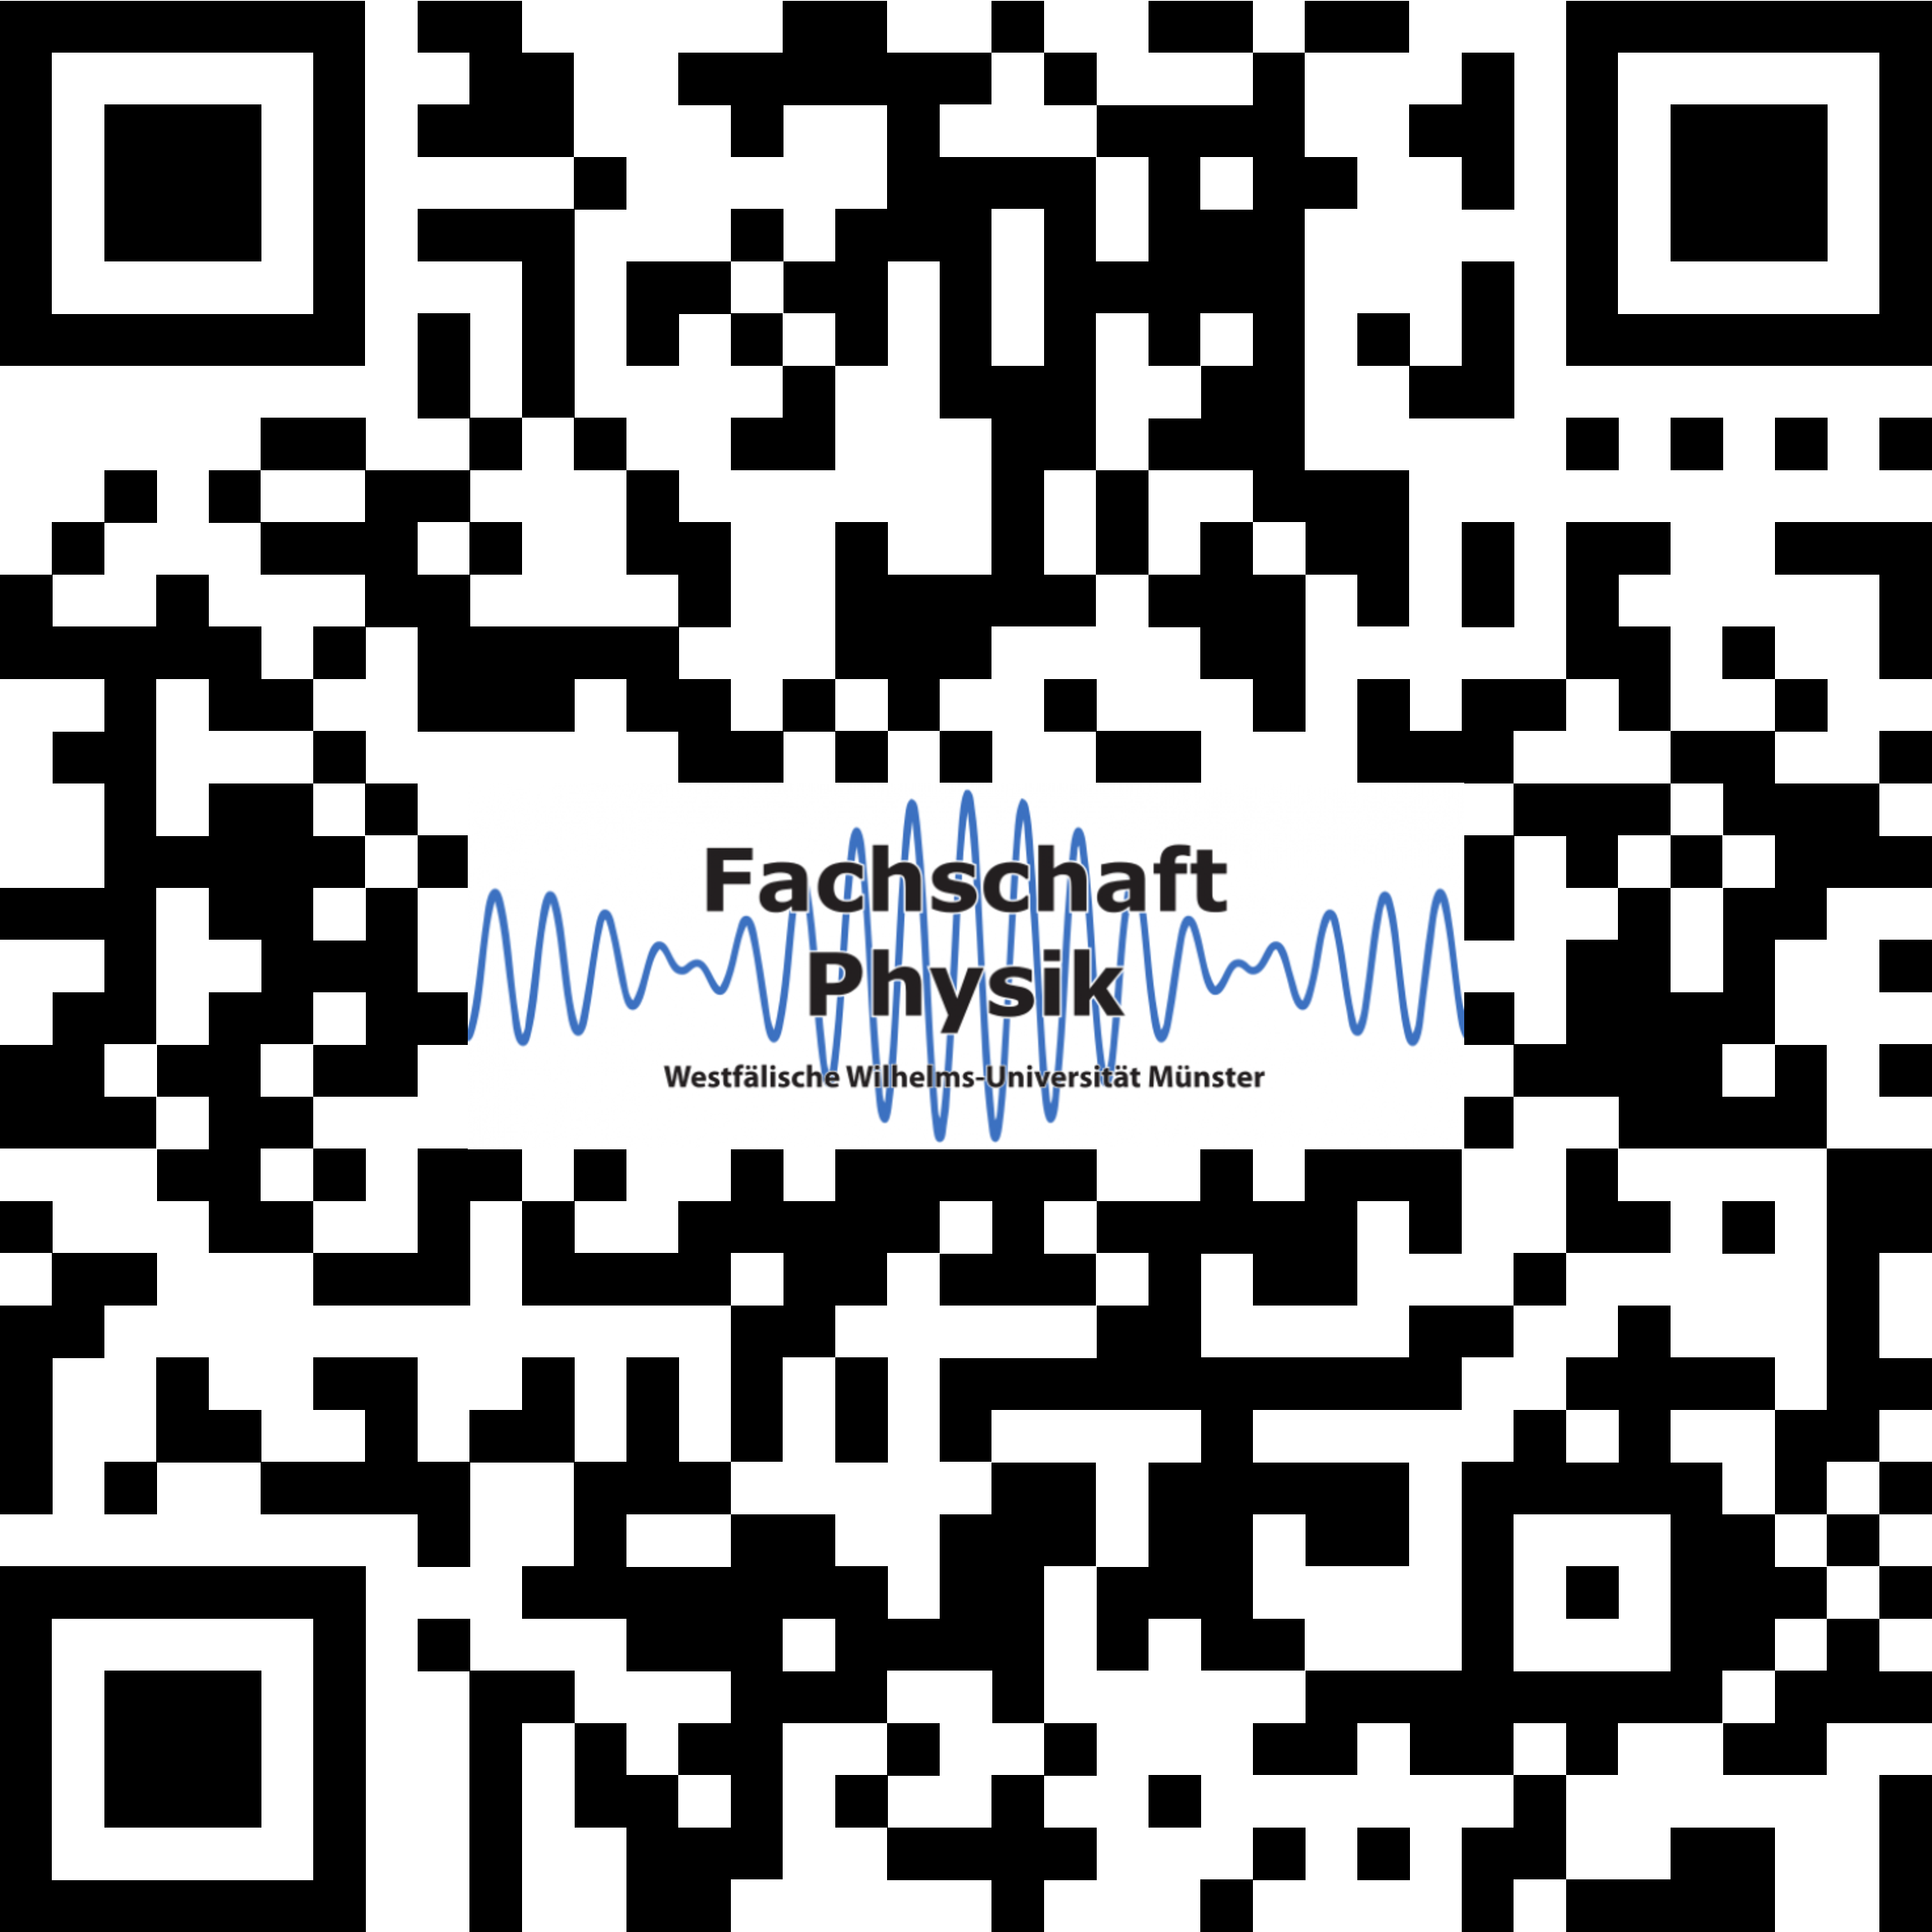
\includegraphics[width=3.8cm]{res/fsphys_qrcode_homepage.png}
		\scriptsize
		\href{https://www.uni-muenster.de/Physik.FSPHYS/}{\texttt{uni-muenster.de/Physik.FSPHYS}}
	\end{minipage}
	\hfill
	\begin{minipage}[t]{4cm}
		% Rechtsbündig und mit etwas Abstand zwischen Paragraphen
		\raggedleft\parskip=0.1cm
		\textbf{Facebook-Seite:}
	
		\includegraphics[width=3.8cm]{res/fsphys_qrcode_facebook.png}
		\scriptsize
		\href{https://facebook.com/fsphys}{\texttt{facebook.com/fsphys}}
	\end{minipage}
\end{minipage}
\end{multicols}
\vfill
\begin{center}
	\vspace{-2mm}
	\includegraphics[width=\columnwidth, height=0.42\textheight]{res/fsphys_gruppenfoto_2018_cropped.jpg}
\end{center}

